\documentclass[a4paper]{article}

\usepackage[pdftex]{graphicx}
\usepackage[margin=3cm]{geometry}
\usepackage{verbatim,moreverb,amssymb,amsmath}


\newcounter{question}
\newcommand{\question}[1]{\refstepcounter{question}\section*{Question~\thequestion~~~\small\emph{(#1)}}}
\renewcommand*\thequestion{\arabic{question}}


\begin{document}

\pagestyle{empty}
\thispagestyle{empty}



\noindent
\begin{minipage}{\columnwidth}
  \centering
  \Large
  DA4002 (HT11) Halmstad University\\
  Introduction to Algorithms, Data Structures, and Problem Solving\\[3\baselineskip]
  \Huge
  Written Exam\\
  \Large
  Tuesday, August 21, 2012\\[2\baselineskip]
  Examiner: Roland Philippsen
\end{minipage}

\vfill

\noindent
\begin{center}
\fbox{
  \begin{minipage}{0.8\columnwidth}
    \textbf{Student Name:}\\[3\baselineskip]
  \end{minipage}
}
\end{center}

\vfill



\section*{Rules}

Aside from the obvious rules of conduct exams (e.g.\ no chatting):

\begin{itemize}
\item
  \textbf{No computing devices} (laptops, phones, calculators, \emph{etc}).
\item
  \textbf{No books or printouts}.
\item
  \textbf{Allowed self-written notes}: two sheets of A4 paper (front and back).
\end{itemize}



\section*{General Guidelines}

\begin{itemize}
\item
  \textbf{Read carefully} and pace yourself.
  You can solve the problems in any order you want, but later problems may be easier to solve after you have answered the preceding questions.
\item
  \textbf{Write clearly} and draw clear diagrams.
  If you need to correct a mistake, then cleanly cross out the wrong answer and clearly indicate where the correction can be found.
\item
  \textbf{Indicate the question number} for each of your answers.
  If a question has sub-questions, indicate the sub-question number after the main question number, separated by a dot.
  For example, question 3 has 4 sub-questions, and their answers should be numbered 3.1, 3.2, 3.3, and 3.4.
\end{itemize}



\pagebreak
\pagestyle{plain}
\thispagestyle{plain}
\setcounter{page}{1}



\question{4 points}

Consider the following four pseudo-code fragments A, B, C, and D:\\

\small
\noindent
\begin{minipage}[t]{0.44\columnwidth}
  
  \begin{tabbing}
    \quad\=\quad\=\quad\=\quad\=\quad\=\kill
    function \textbf{fragmentA} (\emph{arr}, \emph{len}):\\
    \>// \emph{arr} is an array of numbers\\
    \>// \emph{len} is the length of the array\\
    \>for \emph{i} in 0\ldots\emph{len}-1:\\
    \>\>for \emph{j} in 1\ldots\emph{len}-1:\\
    \>\>\>if \emph{arr}[\emph{j}] $<$ \emph{arr}[\emph{j-1}] then\\
    \>\>\>\>swap \emph{arr}[\emph{j}] with \emph{arr}[\emph{j-1}]\\
    \>\>\>end if\\
    \>\>end for\\
    \>end for\\
    end function
  \end{tabbing}
  
  \begin{tabbing}
    \quad\=\quad\=\quad\=\quad\=\quad\=\kill
    function \textbf{fragmentC} (\emph{start})\\
    \>// - \emph{start} is a node\\
    \>// variables:\\
    \>// - \emph{open} is a queue of nodes\\
    \>// - \emph{closed} is a set of nodes\\
    \>// - \emph{it} and \emph{nb} are nodes\\
    \>\emph{open}.push(\emph{start})\\
    \>while \emph{open} is not empty:\\
    \>\>\emph{it} = \emph{open}.pop()\\
    \>\>if \emph{closed} does not contain \emph{it} then\\
    \>\>\>\emph{closed}.add(\emph{it})\\
    \>\>\>for \emph{nb} in \emph{it}.neighbors:\\
    \>\>\>\>if \emph{closed} does not contain \emph{nb} then\\
    \>\>\>\>\>\emph{nb}.predecessor = \emph{it}\\
    \>\>\>\>\>\emph{open}.push(\emph{nb})\\
    \>\>\>\>end if\\
    \>\>\>end for\\
    \>\>end if\\
    \>end while\\
    end function
  \end{tabbing}
  
\end{minipage}%
\hfill%
\begin{minipage}[t]{0.44\columnwidth}
  
  \begin{tabbing}
    \quad\=\quad\=\quad\=\quad\=\quad\=\kill
    function \textbf{fragmentB} (\emph{arr}, \emph{len}, \emph{num}):\\
    \>// - \emph{arr} is an array of numbers\\
    \>// - \emph{len} is the length of the array\\
    \>// - \emph{num} is a number\\
    \>for \emph{i} in 0\ldots\emph{len}-1:\\
    \>\>if \emph{arr}[\emph{i}] $=$ \emph{num} then\\
    \>\>\>return \emph{i}\\
    \>\>end if\\
    \>end for\\
    \>return -1\\
    end function
  \end{tabbing}
  
  \begin{tabbing}
    \quad\=\quad\=\quad\=\quad\=\quad\=\kill
    function \textbf{fragmentD} (\emph{start})\\
    \>// - \emph{start} is a node\\
    \>// NOTE:\\
    \>// \quad someFunction() can be assumed to be given.\\
    \>// \quad It does not matter what that function does,\\
    \>// \quad and it does not modify its argument.\\
    \>someFunction(\emph{start})\\
    \>if \emph{start}.left is not null then\\
    \>\>fragmentD(\emph{start}.left)\\
    \>end if\\
    \>if \emph{start}.right is not null then\\
    \>\>fragmentD(\emph{start}.right)\\
    \>end if\\
    end function
  \end{tabbing}
\end{minipage}
\normalsize
\vspace{\baselineskip}

For each of those code fragments, choose which algorithm name from the table below best corresponds to what the fragment does, and mark its letter \emph{(A, B, C, or D)} in the space on the right.
Mark algorithms which are not shown in any pseudo-code with a big X.

\begin{center}
  \begin{tabular}{|l|p{0.3\columnwidth}|}
    \hline
    \emph{algorithm} & \emph{A, B, C, D, or X} \\
    \hline
    linear search & \\
    \hline
    binary search & \\
    \hline
    sort & \\
    \hline
    pre-order tree traversal & \\
    \hline
    level-order tree traversal & \\
    \hline
    breadth-first graph search & \\
    \hline
  \end{tabular}
\end{center}


\clearpage

\question{4 points}

An array contains \emph{N} numbers, and you want to determine whether two numbers sum to a given number \emph{K}.
For instance, if the input array contains numbers \{8, 4, 1, 6\} and $K = 10$, then the answer is yes (becuase $4 + 6 = 10$).

\begin{enumerate}
\item
  Write the code for a function that performs this task.
\item
  Give an execution time analysis of your method.
\item
  Recall that there are algorithms for sorting arrays that are $O(N \log N)$.
  Use this fact to write a new version of your program that is $O(N \log N)$.
  Proceed by first sorting the array and then doing some linear extra work.
  
  \emph{\underline{Notice:} you do \textbf{not} need to implement sort, assume that it is already implemented.
  Your updated code can simply call a function called \texttt{sort(a)}, where \texttt{a} holds the array.}
\end{enumerate}


\clearpage

\question{3 points}

The ternary number system expresses numbers as sums of powers of 3, in the same way that the decimal system uses powers of 10 and the binary system uses powers of 2.
In ternary, one can use the digits $d_i \in \{0, 1, 2\}$ to compose a number $t$ with $N$ digits using the formula $t = \sum_{i=0}^{N-1} d_i \times 3^i$.
To write a ternary number, the digits are simply stringed together from the most significant $d_{N-1}$ down to the least significant $d_0$.
To illustrate, the following table lists ten numbers written in decimal and ternary:\\

\begin{tabular}{|l|r|r|r|r|r|r|r|r|r|r|}
  \hline
  decimal & 0 & 1 &  2 &  3 &   4 &   5 &   6 &   7 &    8 &   9 \\
  \hline
  ternary & 0 & 1 &  2 & 10 &  11 &  12 &  20 &  21 &   22 &  100 \\
  \hline
\end{tabular}
\vspace{0.5\baselineskip}

Take for example the ternary 12: it has 2 digits, namely $d_1=1$ and $d_0=2$.
Substituting these into the general formula above yields $t = d_1 \times 3^1 + d_0 \times 3^0 = 1 \times 3 + 2 \times 1 = 5$.

\begin{enumerate}
\item
  Write a \emph{recursive} function that prints a given number in ternary.
  In other words, your function should take a single number as argument, and convert it to a string of digits that represent that number in ternary.
\item
  What is the Big-Oh runtime complexity of your function, as a function of the number of decimal digits required to express the number?
\end{enumerate}



\clearpage

\question{3 points}

\begin{minipage}[b]{0.6\columnwidth}
  The \emph{Tower of Hanoi} puzzle consists of three rods and a number of disks of different sizes which can slide onto any rod.
  The puzzle starts with the disks in a neat stack in ascending order of size on one rod, the smallest at the top, thus making a conical shape.
  
  The objective of the puzzle is to move the entire stack to another rod, obeying the following rules:
\end{minipage}
\hfill
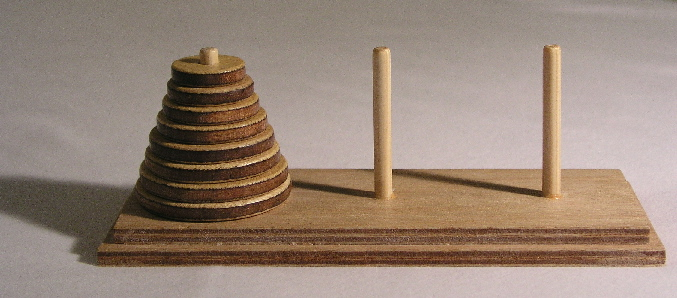
\includegraphics[width=0.35\columnwidth]{Tower_of_Hanoi}

\begin{itemize}
\item
  Only one disk may be moved at a time.
\item
  Each move consists of taking the upper disk from one of the rods and sliding it onto another rod, on top of the other disks that may already be present on that rod.
\item
  No disk may be placed on top of a smaller disk.
\end{itemize}

\footnotesize
\hfill
[Text and photo adapted from Wikipedia.]
\normalsize

\begin{enumerate}
\item
  Write a \emph{recursive} function that prints the moves required to solve the \emph{Tower of Hanoi} puzzle for any number of disks.
  
  The disks are numbered from the top down starting at 1 (the smallest disk) and the three rods are labelled A, B, and C.
  The arguments to your function should be the number of disks, which rod to start from, and which rod to go to.
  The output of your function should look like this (for a stack of 2 disks to move from A to B):
\begin{verbatim}
     disk 1 from A to C
     disk 2 from A to B
     disk 1 from C to B
\end{verbatim}

\item
  Give a mathematical formula for computing the number of moves required to solve the \emph{Tower of Hanoi} puzzle.
  
\end{enumerate}


\clearpage

\question{5 points}

One of your friends is writing an application that frequently has to find out if a number has been encountered before.
Your friend decided to use a binary search tree to store the set of numbers, because of its fast element lookup.
Then a function for saving the set to a file was added, which your friend implemented via in-order tree traversal.
But now, after loading the file, the application runs much slower.

What is going wrong, and how can it be corrected?
Answer the following questions to explain the problem and the solution:
\begin{enumerate}
\item
  Draw a diagram of the binary search tree after the following sequence of numbers has been added to an initially empty tree: 5, 3, 8, 1, 4, 7, 9, 2, 6.
\item
  Write down the sequence of numbers resulting from in-order traversal of that tree.
  Then, draw a diagram of the tree that results when this sequence is added to an initially empty tree.
\item
  Explain why lookups are now slower, and propose a solution to the problem.
\item
  Write down the crucial part of your solution in pseudo-code.
  
  \emph{\underline{Notice:} the solution requires just one function.
    To implement that function you need a queue, which you can assume to be available already (similar to fragment C of question 1).
    You can use Java or the same style of pseudo-code as in question 1.}
\end{enumerate}


\clearpage

\question{6 points}

Answer the following questions about the computational complexity of various algorithms, where $N$ denotes the problem size.\\
\emph{
  \underline{Notice:} you do not need a calculator.
  To help with some of the computations, you can use this convenient lookup table for powers of $2$:}

\begin{tabular}{|l|r|r|r|r|r|r|r|r|r|r|r|r|r|r|r|}
  \hline
  $x=$   & 0 & 1 & 2 & 3 & 4 & 5 & 6 & 7 & 8 & 9 & 10 & 11 & 12 & 13 & 14 \\
  \hline
  $2^x=$ & 1 & 2 & 4 & 8 & 16 & 32 & 64 & 128 & 256 & 512 & 1024 & 2048 & 4096 & 8192 & 16384 \\
  \hline
\end{tabular}

\begin{enumerate}
\item
  Algorithm 1 is known to have a runtime of $T_1(N) = 2 \times N + 0.1 \times N^3 + 50 \times \log(N)$.
  What is its Big-Oh runtime complexity?
\item
  Algorithm 2 is known to be $T_2 \in O(N \log N)$.
  For a sample problem, its runtime has been measured to be $T_2(N=16) = 6.4s$.
  What runtime should be expected for $N=32$?
\item
  Algorithm 3 has exponential runtime complexity.
  For a sample problem of size $5$ it requires $0.32s$ to complete.
  How big of a problem can be expected to be completed in $10.24s$?
\item
  What is the runtime $T_4(N)$ and the Big-Oh complexity of \texttt{function4} in the following Java code fragment?
  Note that the method \texttt{f\_1ms} always requires $1ms$ to run, and the method \texttt{f\_3ms} always takes $3ms$.\\
  \textbf{\emph{CORRECTION:} there was a copy-paste error in the version of \texttt{recurse} handed to the students at the exam, so they all got full points regardless of their answer.}
  \small
  \verbatimtabinput{function4.txt}
  \normalsize
\end{enumerate}



\end{document}
